	
\section{Problem \& Motivation}
	Sparse linear algebra is a key component in various scientific simulations
	ranging from quantum physics to fluid and structural mechanics.
	Unfortunately many iterative numerical methods for sparse systems 
	and important building 	blocks of sparse linear algebra feature strong 
	data dependencies rendering them difficult to be parallelized.
	Typically	loop-carried dependencies may occur in
	iterative solvers  or preconditioners (e.g., Kaczmarz, Gauss-Seidel) 
	or write conflicts show up in the parallelization of building blocks such 
	as symmetric sparse matrix vector.
	Scalable, hardware-efficient parallelization of such kernels is known to be a 
	challenge. Multicoloring is a typical approach to enable parallelization
	of iterative solvers with distance-k dependency \eg the 
	red-black gauss-seidel solves the distance-1 dependency problem.
	However most of the standard solutions suffer from low performance
	on modern hardware, are highly problem specific, or require tailored
    sparse matrix storage formats.

	\Acrshort{RACE} addresses these shortcomings by covering ideas from graph traversal
	and multicoloring to ensure data locality, appropriate levels of parallelism,
	and using hardware efficient parallelization schemes. The method is applicable
	to many problems (\ie matrix structures) and general sparse data storage formats.
	
%	In this paper we present a novel approach called \acrshort{RACE} that helps in
%	solving the general distance-k dependency problem for sparse kernels in a
%	hardware efficient manner. The \acrshort{RACE} method is motivated by the
%	shortcomings of multicoloring methods that are frequently used in this scenario.
%	The method works on simple data storage formats
%	like \acrfull{CRS}, and is highly scalable to meet the requirements of 
%	modern CPU based compute nodes. \medskip

\noindent\textbf{Outline}


\noindent	The paper is structured as follows. \Cref{sec:background} describes
	the underlying dependency problems and the conventional
	approaches used to solve such kind of dependencies. \Cref{sec:uniqueness} 
	shows the general issues that occur while using these conventional
	approaches. We then introduce the \acrshort{RACE} method in \Cref{sec:RACE_method},
	its uniqueness	and how its	basic design addresses the problems. 
	In \Cref{sec:results} we compare \acrshort{RACE} performance to
	available standard approaches, and finally apply the \acrshort{RACE}
	method to parallelize an eigenvalue solver provided by \acrshort{MKL}.
	It demonstrates the necessity of the \acrshort{RACE} method to solve 
	large problems that are far beyond the reach of current state-of-the-art
	implementations.
	
	\begin{comment}
	In this paper we present a novel approach called \acrshort{RACE} that helps in
	solving the general distance-k dependency problem for sparse kernels in a
	hardware efficient manner. The \acrshort{RACE} method is motivated by the
	shortcomings of multicoloring methods that are frequently used in this scenario.
	The method uses a recursive level-based approach to find optimal permutations
	while preserving good data locality. A thorough performance analysis shows that
	our method achieves high hardware efficiency on modern multi-core architectures
	and it outperforms traditional \acrfull{MC} and \acrshort{MKL} implementations
	by a factor of 2--2.5$\times$. We are on par with \acrfull{ABMC} method for
	small matrices, while for large matrices we gain almost a factor of
	1.5--2$\times$. Owing to the success of parallel implementations of
	sparse kernels having dependencies we further demonstrate first results
	of parallel iterative FEAST eigen solver using CGMN internal solver.
	\end{comment}


\section{Background \& Related Work} \label{sec:background}
Many numerical methods that come across in sparse linear algebra are hard to 
parallelize due to dependencies. 
%The two main class of dependencies that occur in this field are \DONE
%dependency as in Gauss-Seidel iteration or a \DTWO dependency as they 
%occur in \acrfull{KACZ} or \acrfull{SymmSpMV}. 

\begin{algorithm}[tb]
	\caption{\label{alg:symmSpMV} \acrshort{SymmSpMV} kernel,  $b=Ax$, in \acrshort{CRS} format.}
	\begin{algorithmic}[1]
		\For{$row=1:nrows$}
			\State{$diag\_idx=rowPtr[row]$}
			\State{$b[row] += A[diag\_idx]*x[row]$}
			\For{$idx=rowPtr[row]+1:rowPtr[row+1]$}
				\State{$b[row] += A[idx]*x[col[idx]]$}
				\State{$b[col[idx]] += A[idx]*x[row]$} 
			\EndFor
		\EndFor
	\end{algorithmic}
\end{algorithm}

 
As a typical example for \DTWO dependency problem, we use \acrlong{SymmSpMV},
 in short \acrshort{SymmSpMV}. 
\Cref{alg:symmSpMV} shows the pseudo-code of \acrshort{SymmSpMV} kernel 
for upper triangular matrix stored in \acrfull{CRS} \cite{CRS} format. 
The kernel exploits the symmetry
of the matrix ($A_{ij} = A_{ji}$) to reduce storage size and overall 
memory traffic which is the biggest bottleneck on modern CPUs. 
However \acrshort{SymmSpMV} cannot be parallelized straightforward as two 
different threads working on two different rows in parallel could potentially 
write to the same element ($b[col[idx]]$) of the indirectly accessed $b$ vector
causing write conflicts.
In terms of graph theory this means a vertex (row in a matrix) and 
its \DTWO neighbor \cite{dist_k_def} cannot be operated in parallel.
In this paper we concentrate on such \DTWO dependency problems, although 
the underlying method and library is capable of handling 
general \DK dependencies.


A popular approach to solve such kind of dependency problem are  the
\acrfull{MC} techniques. Earliest work on coloring is the red-black 
Gauss-Seidel scheme~\cite{RBGS}, which was applied to  matrices with
 known sparsity pattern. 
Later \acrlong{MC} techniques have been expanded using graph theory
for general sparse matrices \cite{MC, COLPACK}.
Variants like \acrfull{ABMC} \cite{ABMC} have tried to improve the performance 
of the \acrshort{MC} methods. 
In \cite{feast_mc}, \acrshort{MC} was applied to Kaczmarz iterative solver
having \DTWO dependency.
Specifically to \acrshort{SymmSpMV} there has been no previous attempt to use 
graph based techniques. General solutions for \acrshort{SymmSpMV} are 
locking-based methods and thread-private target arrays \cite{sparseX,thread_private_symm_spmv}.
Depending on the matrix structure these approaches could lead to performance
 degradation  due to serialization and massive increase in data traffic.
Recent researches in this direction use specialized storage formats like
 CSB \cite{CSB} or RSB \cite{RSB} but this requires rewriting of existing 
 code and lots of tuning. 

%to Kaczmarz iterative solver having  dependency. 
 
%Many solution to these dependency problems have been proposed, such as 
%locking method and thread-private target arrays \cite{sparseX,thread_private_symm_spmv}.
%But these approaches could lead to performance degradation depending
%on the matrix due to serialization or increase in data traffic respectively.
%Recent researches include in the direction of special storage formats like
% CSB \cite{CSB} or RSB \cite{RSB} but this require rewriting of existing 
% code and lot of tuning. Another popular approach in the field is matrix 
%reordering technique, on which we focus here.
%One of the earliest work on reordering is the red-black 
%Gauss--Seidel scheme~\cite{RBGS}. 
%Later it has been generalized for sparse matrices and \DK dependent 
%problems by well-known \acrfull{MC} approaches \cite{MC, COLPACK}. 
%Variants like \acrfull{ABMC} \cite{ABMC} have tried to
%improve the  performance of the \acrshort{MC} methods. In \cite{feast_mc},
%\acrshort{MC} was applied to \acrshort{KACZ} kernel having  \DTWO dependency. 

\section{Uniqueness of the Approach} \label{sec:uniqueness}
Approaches like \acrshort{MC} can help in parallelization of kernels like \acrshort{SymmSpMV},
however the method can destroy data locality of the matrix leading to low performance.
%\setlength{\belowcaptionskip}{-12pt}
\begin{figure}[tb]
	\centering
	\subfloat[\label{fig:mc_problem_a} Original ordering]{\scalebox{0.625}{%\documentclass{standalone}
%\usepackage{tikz}

%\begin{document}

%\begin{minipage}{0.55\textwidth}
%	\centering
	\def\rowperm{{0, 1, 2, 3, 4, 5, 6}}
	%\def\colperm{{0, 1, 2, 3, 4, 5, 6}}
	\def\colperm{{0, 1, 2, 3, 4, 5, 6}}
	\scalebox{0.7}{\begin{tikzpicture}
		\foreach \x in {0,1}
		\fill[gray] (\colperm[\x]-1,6) rectangle (\colperm[\x],7);
		\foreach \y in {0,1,2,3,4}  
			\foreach \x in {0,1,2}
				\fill[gray] (\colperm[\x]-1+\y,5-\y) rectangle (\colperm[\x]+\y,6-\y);   
		\foreach \x in {0,1}
			\fill[gray] (\colperm[5+\x]-1,0) rectangle (\colperm[5+\x],1); 	
		\draw[step=1cm,black,very thin] (-1,-0) grid (6,7);
		\end{tikzpicture}}
	\hspace{0.3cm}
	\scalebox{0.7}{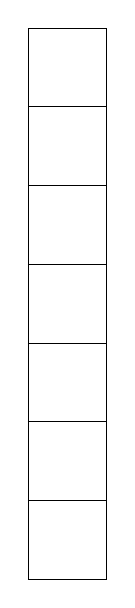
\begin{tikzpicture}
		\draw[step=1cm,black,very thin] (8,-0) grid (9,7);
	\end{tikzpicture}}

%\end{minipage}
%\end{document}
}}\hspace{0.5em}
	\subfloat[After \acrshort{MC} applied]{\label{fig:mc_problem_b} \scalebox{0.625}{%\end{minipage}
\def\rowperm{{0, 1, 2, 3, 4, 5, 6}}
%\def\colperm{{0, 1, 2, 3, 4, 5, 6}}
\def\colperm{{0, 1, 2, 3, 4, 5, 6}}
%\begin{minipage}{0.55\textwidth}
%\centering
\scalebox{0.7}{\begin{tikzpicture}
	\foreach \x in {0,1}
	\fill[red!65!white] (\colperm[\x]-1,6) rectangle (\colperm[\x],7);  
	\foreach \x in {0,1,2}
	\fill[red!65!white] (\colperm[2+\x]-1,5) rectangle (\colperm[2+\x],6);   
	\foreach \x in {0,1}
	\fill[red!65!white] (\colperm[5+\x]-1,4) rectangle (\colperm[5+\x],5); 

	\node at (\colperm[0]-0.5,6.5) {\Large{1}}; 
	\node at (\colperm[1]-0.5,6.5) {\Large{1}}; 
	\node at (\colperm[2]-0.5,5.5) {\Large{2}}; 
	\node at (\colperm[3]-0.5,5.5) {\Large{2}}; 
	\node at (\colperm[4]-0.5,5.5) {\Large{2}}; 
	\node at (\colperm[5]-0.5,4.5) {\Large{3}}; 
	\node at (\colperm[6]-0.5,4.5) {\Large{3}}; 
	
	\foreach \x in {0,1,2}
	\fill[green!65!white] (\colperm[\x]-1,3) rectangle (\colperm[\x],4);  
	\foreach \x in {0,1,2}
	\fill[green!65!white] (\colperm[3+\x]-1,2) rectangle (\colperm[3+\x],3);   
	\draw[step=1cm,gray,very thin] (-1,-0) grid (6,7);
	\node at (\colperm[0]-0.5,3.5) {\Large{1}}; 
	\node at (\colperm[1]-0.5,3.5) {\Large{1}}; 
	\node at (\colperm[2]-0.5,3.5) {\Large{1}}; 
	\node at (\colperm[3]-0.5,2.5) {\Large{2}}; 
	\node at (\colperm[4]-0.5,2.5) {\Large{2}}; 
	\node at (\colperm[5]-0.5,2.5) {\Large{2}}; 
	
	\foreach \x in {0,1,2}
	\fill[blue!65!white] (\colperm[1+\x]-1,1) rectangle (\colperm[1+\x],2);  
	\foreach \x in {0,1,2}
	\fill[blue!65!white] (\colperm[4+\x]-1,0) rectangle (\colperm[4+\x],1);
	\draw[step=1cm,gray,very thin] (-1,-0) grid (6,7);   
	
	\node at (\colperm[1]-0.5,1.5) {\Large{1}}; 
	\node at (\colperm[2]-0.5,1.5) {\Large{1}}; 
	\node at (\colperm[3]-0.5,1.5) {\Large{1}}; 
	\node at (\colperm[4]-0.5,0.5) {\Large{2}}; 
	\node at (\colperm[5]-0.5,0.5) {\Large{2}}; 
	\node at (\colperm[6]-0.5,0.5) {\Large{2}}; 
	\draw[step=1cm,black,very thin] (-1,-0) grid (6,7);
\end{tikzpicture}}
\hspace{0.3cm}
\scalebox{0.7}{\begin{tikzpicture}
	\foreach \x in {0,1,2,3,4,5,6}
	\fill[red!65!white] (8,\x) rectangle (9,\x+1);  
	\draw[step=1cm,black,very thin] (8,-0) grid (9,7);
	\node at (8.5,6.5-\colperm[0]) {\Large{1}}; 
	\node at (8.5,6.5-\colperm[1]) {\Large{1}}; 
	\node at (8.5,6.5-\colperm[2]) {\Large{2}}; 
	\node at (8.5,6.5-\colperm[3]) {\Large{2}}; 
	\node at (8.5,6.5-\colperm[4]) {\Large{2}}; 
	\node at (8.5,6.5-\colperm[5]) {\Large{3}}; 
	\node at (8.5,6.5-\colperm[6]) {\Large{3}}; 
\end{tikzpicture}}
%\end{minipage}
%\end{document}
}}
	%	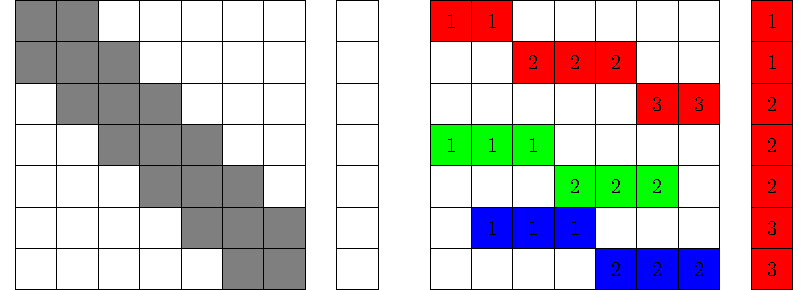
\includegraphics[scale=0.6]{pics/alpha_problem/mc_alpha_unsymm_only_red.tex}
	\caption{\label{fig:mc_problem} Illustration of data locality degradation due to \acrshort{MC}.
		Numbers represent thread id}
\end{figure}
\begin{figure}[b]
	\subfloat[Scaling performance]{\label{fig:motivation_symm_spmv}\scalebox{0.8}{\pgfplotsset{width=5.5cm,height=7.25cm,compat=1.3}
\def\matrixFile{pics/Spin-26/data}
\def\matrix{Spin-26}
\def\matrixName{Spin-26 }
\pgfplotstableread[col sep=comma] {\matrixFile/MKL/\matrix/spmv.txt} \SPMV
\pgfplotstableread[col sep=comma] {\matrixFile/MC_RCM/\matrix/symm_spmv.txt} \SYMMSPMVMC
\pgfplotstableread[col sep=comma] {\matrixFile/ABMC_RCM/\matrix/symm_spmv.txt} \SYMMSPMVABMC
\pgfplotstableread[col sep=comma] {\matrixFile/RACE/\matrix/symm_spmv.txt} \SYMMSPMVRACE
\pgfplotstableread[col sep=space] {\matrixFile/nnz} \NNZfile

\pgfplotstablegetelem{0}{nnz}\of\NNZfile
\pgfmathsetmacro{\NNZ}{\pgfplotsretval}

\newcommand{\rlmCopy}{7.627}
\newcommand{\rlmLoad}{8.962}
\begin{tikzpicture}[tight background]


\def\xmin{0}
\def\xmax{10}
\def\ymin{0}
\def\ymax{30}

\begin{axis}[ xlabel={Threads}, ylabel={Performance (GF/s)}, ymode=linear,
x tick label style={font={\Large}},
y tick label style={font={\Large}},
%xtick={1000, 2744, 5832, 10648, 17576, 27000, 39304, 54872, 74088},
%xticklabels={$10^3$, %$14^3$
%  , $18^3$, $22^3$, $26^3$, $30^3$, $34^3$, $38^3$, $42^3$},
scaled ticks=false,
%xmode=log,
xmin=0,xmax = 10,
ymin=0,
ymax=9.9,
%xlabel style={xshift=0.75em},
%ymin=0, ymax=14,
legend style={legend pos=north west, font=\footnotesize}]

%\addplot+[line width=2, color=magenta, mark options={magenta}] table[x =THREAD,y =PERF (GFlop/s),col sep=comma] {\SPMV}; \label{plot_one}
%\addlegendentry{SpMV}

\addplot+[line width=2, color=green, mark options={green}] table[x =THREAD,y =PERF (GFlop/s),col sep=comma] {\SYMMSPMVMC}; \label{plot_two}
\addlegendentry{SymmSpMV MC}

\addplot+[line width=2, color=cyan, mark options={cyan}] table[x =THREAD,y =PERF (GFlop/s),col sep=comma] {\SYMMSPMVABMC}; \label{plot_three}
\addlegendentry{SymmSpMV ABMC}

\addplot+[line width=2, color=orange, mark options={orange}] table[x =THREAD,y =PERF (GFlop/s),col sep=comma] {\SYMMSPMVRACE}; \label{plot_four}
\addlegendentry{SymmSpMV RACE}

%\addplot+[name path=RLM-copy, mark=square*, mark options={red}, draw=red] coordinates {(1,\rlmCopy) (6, \rlmCopy) (8, \rlmCopy) (10, \rlmCopy)}; \label{plot_five}
%\addlegendentry{Ideal}
  

\end{axis}
\end{tikzpicture}
}}\hspace{0.5em}
	\subfloat[Data traffic]{\label{fig:motivation_data}\scalebox{0.8}{\documentclass{standalone}
\usepackage{tikz}
\usepackage{pgfplots}
\pgfplotsset{width=15cm,height=12cm,compat=1.3}
\usepackage{filecontents}
\usetikzlibrary{patterns}
\usepackage{pgfplotstable}

\def\matrixFile{../data/}
\def\matrix{Spin-26}
\def\matrixName{Spin-26 }
\newcommand{\ideal}{11.25}

\begin{document}
	\pgfplotstableread[col sep=comma] {\matrixFile/MKL/\matrix/spmv.txt} \SPMV
	\pgfplotstableread[col sep=comma] {\matrixFile/MC_RCM/\matrix/spmv.txt} \SPMVMC
	\pgfplotstableread[col sep=comma] {\matrixFile/MC_RCM/\matrix/symm_spmv.txt} \SYMMSPMVMC
	\pgfplotstableread[col sep=comma] {\matrixFile/ABMC_RCM/\matrix/spmv.txt} \SPMVABMC
	\pgfplotstableread[col sep=comma] {\matrixFile/ABMC_RCM/\matrix/symm_spmv.txt} \SYMMSPMVABMC
	\pgfplotstableread[col sep=comma] {\matrixFile/RACE/\matrix/symm_spmv.txt} \SYMMSPMVRACE
	\pgfplotstableread[col sep=space] {\matrixFile/nnz} \NNZfile
		
	\pgfplotstablegetelem{0}{nnz}\of\NNZfile
	\pgfmathsetmacro{\NNZ}{\pgfplotsretval}
		
	
		\begin{tikzpicture}
		\begin{axis}[
		width  = 12cm,
		height = 11cm,
		major x tick style = transparent,
		minor ytick={1, 5, 10, 15, 20, 25, 30 ,35,40},
		grid = minor,
		ybar=2*\pgflinewidth,
		bar width=16pt,
		ymajorgrids = true,
		grid style={dashed, gray!40},
		ylabel = {\Large{Bytes/NNZ}},
		symbolic x coords={SpMV, SymmSpMV-MC, SymmSpMV-ABMC},
		x tick label style={rotate=25,font={\large}},
		y tick label style={font={\Large}},
		xtick = data,
		scaled y ticks = false,
		enlarge x limits=0.25,
		ymin=0,% ymax=42,
		legend cell align=left,
		legend style={
			%at={(1,1.05)},
			%anchor=south east,
			%column sep=1ex,
			legend pos=north west
		},
		]
		

		\pgfkeys{/pgf/fpu}

		\pgfplotstablegetelem{9}{MEM (GB)}\of\SPMV
		\pgfmathsetmacro{\memSPMV}{\pgfplotsretval*1*1/(\NNZ*0.5*1e-8)} %change to SpMV
		\pgfplotstablegetelem{9}{MEM (GB)}\of\SPMVMC
		\pgfmathsetmacro{\memSPMVMC}{\pgfplotsretval*1*1/(\NNZ*0.5*1e-8)}
		\pgfplotstablegetelem{9}{MEM (GB)}\of\SPMVABMC
		\pgfmathsetmacro{\memSPMVABMC}{\pgfplotsretval*1*1/(\NNZ*0.5*1e-8)}
		\pgfplotstablegetelem{9}{MEM (GB)}\of\SYMMSPMVMC
		\pgfmathsetmacro{\memSYMMSPMVMC}{\pgfplotsretval*1*1/(\NNZ*0.5*1e-8)}
		\pgfplotstablegetelem{9}{MEM (GB)}\of\SYMMSPMVABMC
		\pgfmathsetmacro{\memSYMMSPMVABMC}{\pgfplotsretval*1*1/(\NNZ*0.5*1e-8)}
		\pgfplotstablegetelem{9}{MEM (GB)}\of\SYMMSPMVRACE
		\pgfmathsetmacro{\memSYMMSPMVRACE}{\pgfplotsretval*1*1/(\NNZ*0.5*1e-8)}
		
		\addplot[pattern=horizontal lines]%style={ppurple,fill=ppurple}]
		coordinates {(SpMV,\memSPMV) (SymmSpMV-MC,\memSYMMSPMVMC) (SymmSpMV-ABMC,\memSYMMSPMVABMC)};

		\pgfplotstablegetelem{9}{L3 (GB)}\of\SPMV
		\pgfmathsetmacro{\memSPMV}{\pgfplotsretval*1*1/(\NNZ*0.5*1e-8)} %change to SpMV
		\pgfplotstablegetelem{9}{L3 (GB)}\of\SPMVMC
		\pgfmathsetmacro{\memSPMVMC}{\pgfplotsretval*1*1/(\NNZ*0.5*1e-8)}
		\pgfplotstablegetelem{9}{L3 (GB)}\of\SPMVABMC
		\pgfmathsetmacro{\memSPMVABMC}{\pgfplotsretval*1*1/(\NNZ*0.5*1e-8)}
		\pgfplotstablegetelem{9}{L3 (GB)}\of\SYMMSPMVMC
		\pgfmathsetmacro{\memSYMMSPMVMC}{\pgfplotsretval*1*1/(\NNZ*0.5*1e-8)}
		\pgfplotstablegetelem{9}{L3 (GB)}\of\SYMMSPMVABMC
		\pgfmathsetmacro{\memSYMMSPMVABMC}{\pgfplotsretval*1*1/(\NNZ*0.5*1e-8)}
		\pgfplotstablegetelem{9}{L3 (GB)}\of\SYMMSPMVRACE
		\pgfmathsetmacro{\memSYMMSPMVRACE}{\pgfplotsretval*1*1/(\NNZ*0.5*1e-8)}

		\addplot[fill=gray!180]%style={ppurple,fill=ppurple}]
		coordinates {(SpMV,\memSPMV) (SymmSpMV-MC,\memSYMMSPMVMC) (SymmSpMV-ABMC,\memSYMMSPMVABMC)};

		\pgfplotstablegetelem{9}{L2 (GB)}\of\SPMV
		\pgfmathsetmacro{\memSPMV}{\pgfplotsretval*1*1/(\NNZ*0.5*1e-8)} %change to SpMV
		\pgfplotstablegetelem{9}{L2 (GB)}\of\SPMVMC
		\pgfmathsetmacro{\memSPMVMC}{\pgfplotsretval*1*1/(\NNZ*0.5*1e-8)}
		\pgfplotstablegetelem{9}{L2 (GB)}\of\SPMVABMC
		\pgfmathsetmacro{\memSPMVABMC}{\pgfplotsretval*1*1/(\NNZ*0.5*1e-8)}
		\pgfplotstablegetelem{9}{L2 (GB)}\of\SYMMSPMVMC
		\pgfmathsetmacro{\memSYMMSPMVMC}{\pgfplotsretval*1*1/(\NNZ*0.5*1e-8)}
		\pgfplotstablegetelem{9}{L2 (GB)}\of\SYMMSPMVABMC
		\pgfmathsetmacro{\memSYMMSPMVABMC}{\pgfplotsretval*1*1/(\NNZ*0.5*1e-8)}
		\pgfplotstablegetelem{9}{L2 (GB)}\of\SYMMSPMVRACE
		\pgfmathsetmacro{\memSYMMSPMVRACE}{\pgfplotsretval*1*1/(\NNZ*0.5*1e-8)}
				
		\addplot[pattern=vertical lines]%style={ppurple,fill=ppurple}]
		coordinates {(SpMV,\memSPMV) (SymmSpMV-MC,\memSYMMSPMVMC) (SymmSpMV-ABMC,\memSYMMSPMVABMC)};
	
		
		\pgfkeys{/pgf/fpu=false}

		\addplot[draw=red,smooth,dashed, line width=3pt] coordinates { (SymmSpMV-MC,\ideal) (SymmSpMV-ABMC,\ideal)};
				
		\legend{MEM, L3, L2, Ideal SymmSpMV}
		\end{axis}
	%	\node at (6.5,10) {Data traffic Comparison using LIKWID};
		\end{tikzpicture}
\end{document}
}}
	\caption{\label{fig:motivation}(a) Performance of \acrshort{SymmSpMV} with 
		\acrshort{MC} and \acrshort{ABMC} compared to \acrshort{RACE}. 
		(b) Average main memory data traffic in bytes (B) per nonzero entry ($\acrshort{nnz}$) 
		of the full matrix as measured with \LIKWID tool \cite{LIKWID}. The ideal data traffic
		as predicted by performance model is shown for reference.}
\end{figure}
The reason for this is the nature of \acrlong{MC} 
permutation. For \DTWO coloring, \acrshort{MC}
groups rows that do not overlap in any column 
entries \cite{dist_k_def} (structurally orthogonal rows).
 These groups of rows are referred to as colors. 
 Due to this grouping one can parallelize all the rows in a color.
In the \acrshort{SymmSpMV} example (see \cref{alg:symmSpMV}) 
threads within a color operate on different rows having entirely different 
$col[idx]$ avoiding write conflicts in $b$ vector. \Cref{fig:mc_problem}
shows an illustration of a matrix before (\Cref{fig:mc_problem_a}) and 
after (\Cref{fig:mc_problem_b}) applying \acrshort{MC} permutation.
Observe that within a color (for \eg red) none of the rows share same column index.
As the matrix is traversed row by row (see \cref{alg:symmSpMV}) the original matrix
has good data locality and most of the indirect accesses to the vector 
correspond to nearby elements that were loaded in the computation of previous rows.
This ensures the  vector needs to be transferred only
once from the main memory, and the rest of the accesses are from 
fast caches. However coloring the matrix destroys this data locality. For example
in \Cref{fig:mc_problem_b} computing all the red colored rows leads to loading the 
vector completely. If the cache holds only  six elements, 
computation on green and blue rows require loading almost the entire vector again 
from the slow main memory. 

%The matrix after multicoloring permutation is seen in \Cref{fig:mc_problem_b},
%observe that within a color (for \eg red) none of the rows share same column entry. 
%Traversing the elements of the original matrix row by row, would require only 
%one time loading of the right-hand-side (RHS) vector entry, as the elements 
% carried out on
% a matrix (see \Cref{fig:mc_problem_a}) that initially has high data locality.


The data locality along with secondary effects of coloring like 
synchronization costs and false sharing lead to performance degradation.
To demonstrate this we present in \Cref{fig:motivation} performance and 
data transfer volumes of \acrshort{SymmSpMV} computation using various coloring methods.
The experiment was done on \texttt{Spin-26} \cite{Spin} matrix taken from quantum physics application
and the hardware was one socket of \Intel \IVB (E5-2660 v2) clocked at 2.2\,\GHZ.
\Cref{fig:motivation_data} shows the average main memory data traffic per non-zero  of the 
general matrix during \acrshort{SymmSpMV} execution. It can be clearly seen that 
the memory traffic is almost  $4 \times$ higher 
for the \acrshort{MC} method compared to ideal traffic (red line) predicted
by performance model\footnote{See \Cref{sec:results} for more details on modeling.}.
The extra data traffic is mainly due to the low data locality and thereby incurred 
extra accesses of the indirectly accessed vectors. 
\Acrfull{ABMC} tries to reduce the memory traffic by first partitioning the matrix
into blocks and then applying coloring. This improves (reduces) the data traffic compared 
to \acrshort{MC} but is still far from optimal in this case. 

As main memory bandwidth is the main bottleneck on modern compute devices,
 this extra traffic reflects directly on the performance.
This is seen in \Cref{fig:motivation_symm_spmv}, where the performance is
shown in giga floating point operations in seconds (\GF). The ideal 
 performance as predicted by performance model is $\approx 7.6\,\GF$ (not shown in figure)
 for this matrix, but \acrshort{MC} and \acrshort{ABMC} are well below this limit.
 However with our \acrshort{RACE} method both the data traffic and performance 
 remains close to the ideal case, hence having a speed-up of almost
  $4\times$ compared to other methods.


\begin{comment}
\Cref{fig:motivation_symm_spmv} shows performance in giga floating point 
operations per second (\GF) as a function of thread (core).
The general variant  of sparse matrix-vector multiplication (\acrshort{SpMV})
 using the full matrix  serves as the yardstick for comparison. 
Based on a naive performance analysis, as most of the sparse
kernels are highly memory bound on modern architectures
one would expect \acrshort{SymmSpMV} performance 
to be almost twice that of \acrshort{SpMV}, due to half the data traffic. 
However the \acrshort{SymmSpMV} implementation using \acrshort{MC} is more
than three times slower.
\end{comment}

\section{RACE Method} \label{sec:RACE_method}
The \acrshort{RACE} method is designed by  keeping the shortcomings
of coloring approaches in mind. The idea is to have a general hardware 
friendly approach applicable even for simple matrix storage formats 
like \acrshort{CRS}.
\Acrshort{RACE} method consists of three steps:
\begin{enumerate}
	\item level construction
	\item \DK coloring
	\item load balancing
\end{enumerate}
Depending on the matrix and hardware the steps are applied recursively 
if required. 
To illustrate the method we choose a
simple matrix which is associated with an artificially constructed
two-dimensional-seven-point (2d-7pt) stencil. \Cref{fig:orig_graph} shows
the corresponding graph and the sparsity pattern (in inset) of the matrix.

In this paper we restrict ourselves to matrices representing strongly connected 
undirected graphs.

\subsection{Level Construction}
In the first step we determine different levels of a graph and permute the data structure.
This we achieve using well-known bandwidth reduction algorithms like \Acrfull{RCM}\cite{RCM}
or \Acrfull{BFS}\cite{BFS}. Although \acrshort{RCM} is implemented in \acrshort{RACE},
in the following we use \acrshort{BFS} reordering for simpler illustration. 

% \setlength{\belowcaptionskip}{0pt}
\begin{figure}[tb]
	\subfloat[Original graph]{\label{fig:orig_graph}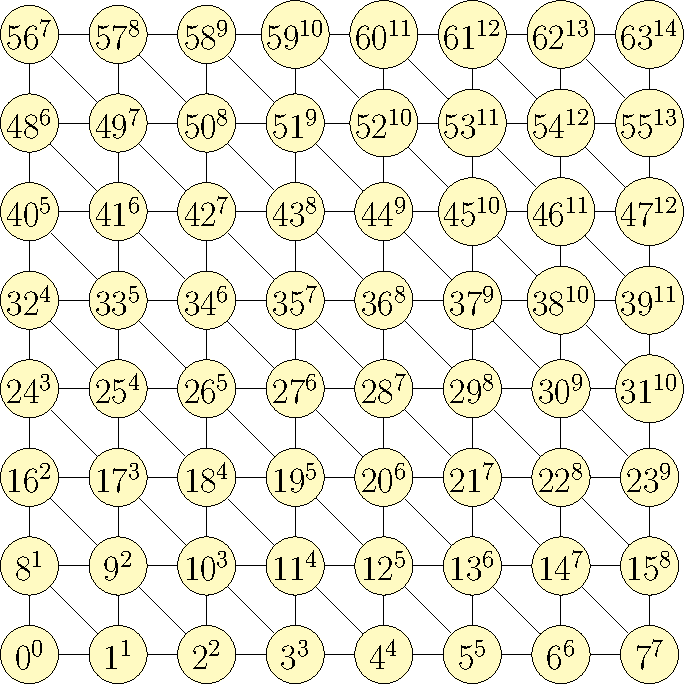
\includegraphics[scale=0.32]{pics/race_method/orig_graph}
		\begin{picture}(0,0)
		\put(-42.5,65.5){{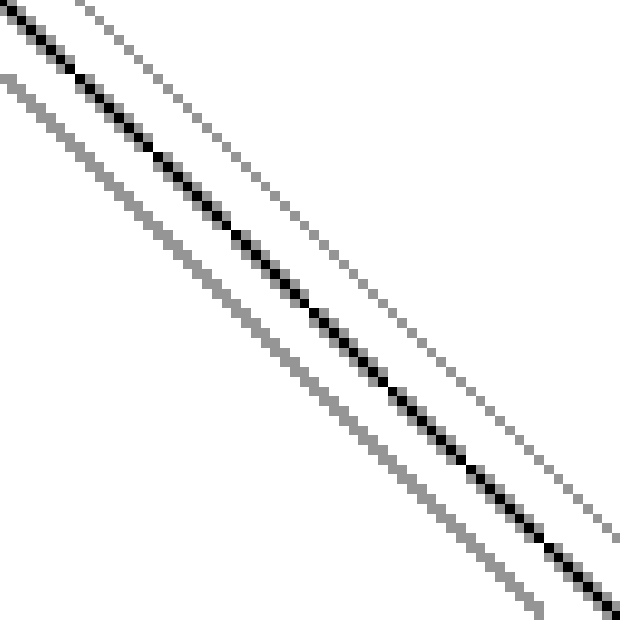
\includegraphics[scale=0.065]{pics/race_method/orig_matrix}}}
		\end{picture}
	}
	\subfloat[Permuted graph]{\label{fig:perm_graph}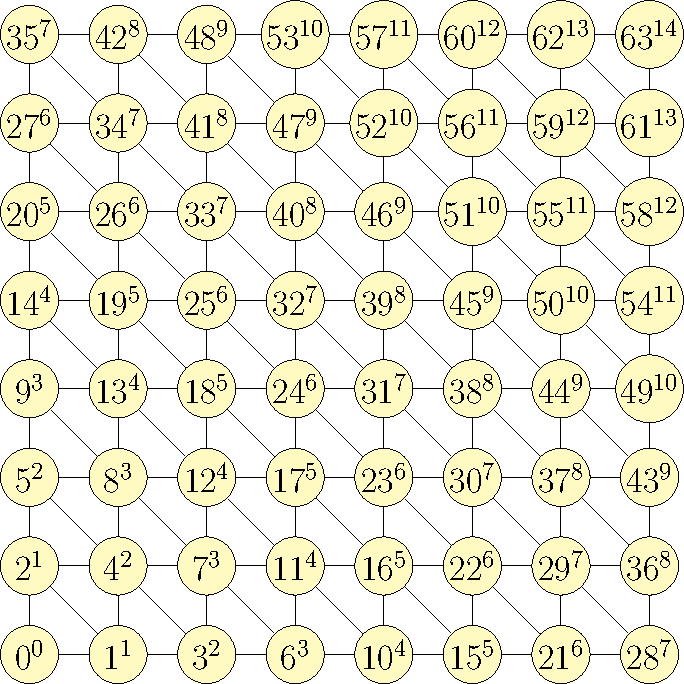
\includegraphics[scale=0.32]{pics/race_method/perm_graph}
		\begin{picture}(0,0)
		\put(-42.5,65.5){{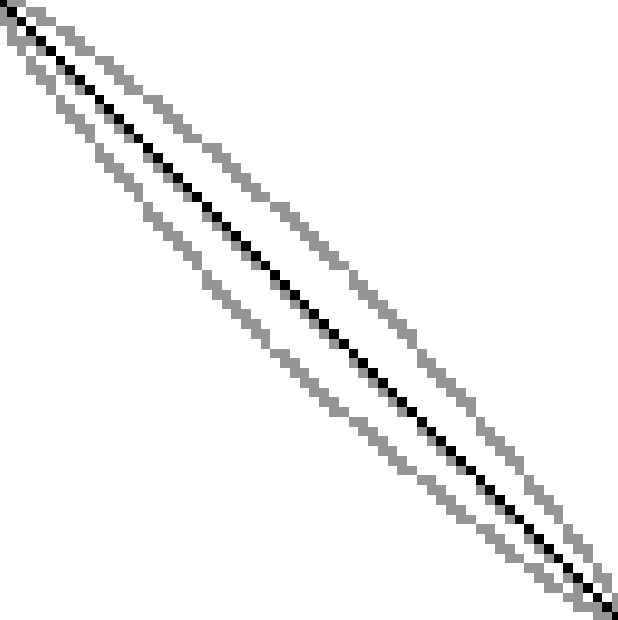
\includegraphics[scale=0.065]{pics/race_method/perm_matrix}}}
		\end{picture}
	}
	\subfloat[]{\label{fig:levelPtr}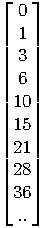
\includegraphics[scale=0.95]{pics/race_method/levelPtr}
		}
	\caption{\label{fig:level_construction}(a) shows the original graph of 2d-7pt example, domain size $8 \times 8$  and (b) shows the graph after applying permutation according to levels. The level numbers are denoted on the superscript of the vertices. Figures in inset show the corresponding sparsity pattern of the matrix. \Cref{fig:levelPtr} shows the \levelPtr.}
\end{figure}

 
In this step we first choose a root vertex and assign it to the first level ($L(0)$). 
The next levels $L(i)$ are defined to contain all vertices that are directly related to previous
level $L(i-1)$ but not in $L(i-2)$. This implies $i$-th level consists of all vertices
that have a minimum distance of $i$ from root node. In \Cref{fig:level_construction} the
level numbers ($i$) are denoted in the superscript of the vertices. 

After the levels are determined we permute (reorder) the matrix (and graph) according
to levels such that the vertices in $L(i)$ appear before $L(i+1)$.  \Cref{fig:perm_graph}
shows the graph and matrix after applying the permutation. Note that the vertex numbering 
in permuted graph has changed compared to original matrix, which was lexicographically ordered.
It is well-known  that such permutation increase data locality
of the computations and has been previously applied to for sparse matrix
computations without any dependencies \cite{RCM_Sparse_computation}.

\Inorder to resolve dependencies \acrshort{RACE} additionally stores information
about levels. We do this by storing the index of the first vertex corresponding
to each level in a data structure called \levelPtr (see \Cref{fig:levelPtr}).

\subsection{Distance-k Coloring}
The \DK coloring step uses the information of the \levelPtr created above to resolve
dependencies. Two vertices are called \DK neighbors if the shortest path connecting 
them consists of at most $k$ edges \cite{dist_k_def}. This implies two vertices
 are \DK independent if they are not \DK neighbors. Based on this definition
 it can be proved that vertices between levels $L(i)$ and $L(i \pm (k+j))$ are
 \DK independent, $\forall j\ge1$. The levels that satisfy this criteria
 are called \DK independent levels.
 
 \setlength{\belowcaptionskip}{-8pt}
 \begin{figure}[t]
 	\vspace*{-0.6cm}
 	\subfloat[\DONE coloring]{\label{fig:d1_color}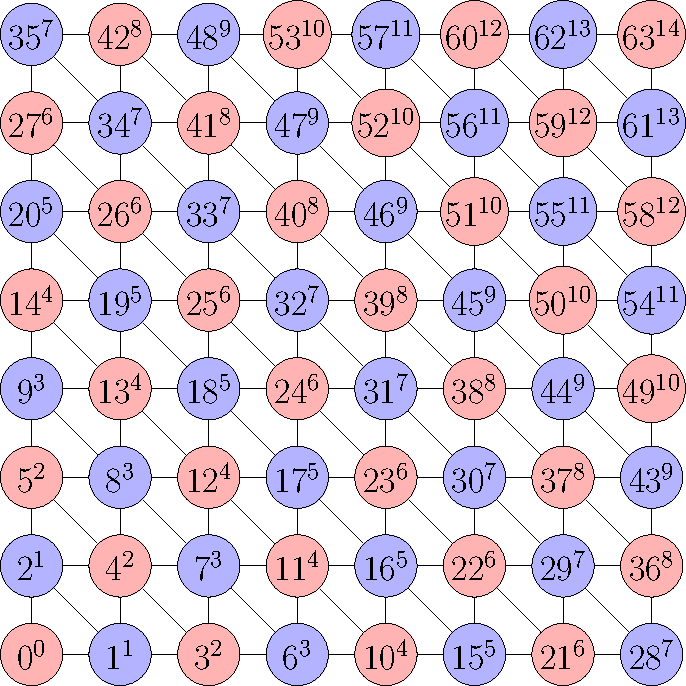
\includegraphics[scale=0.32]{pics/race_method/d1_color}}
 	\subfloat[\DTWO coloring]{\label{fig:d2_color}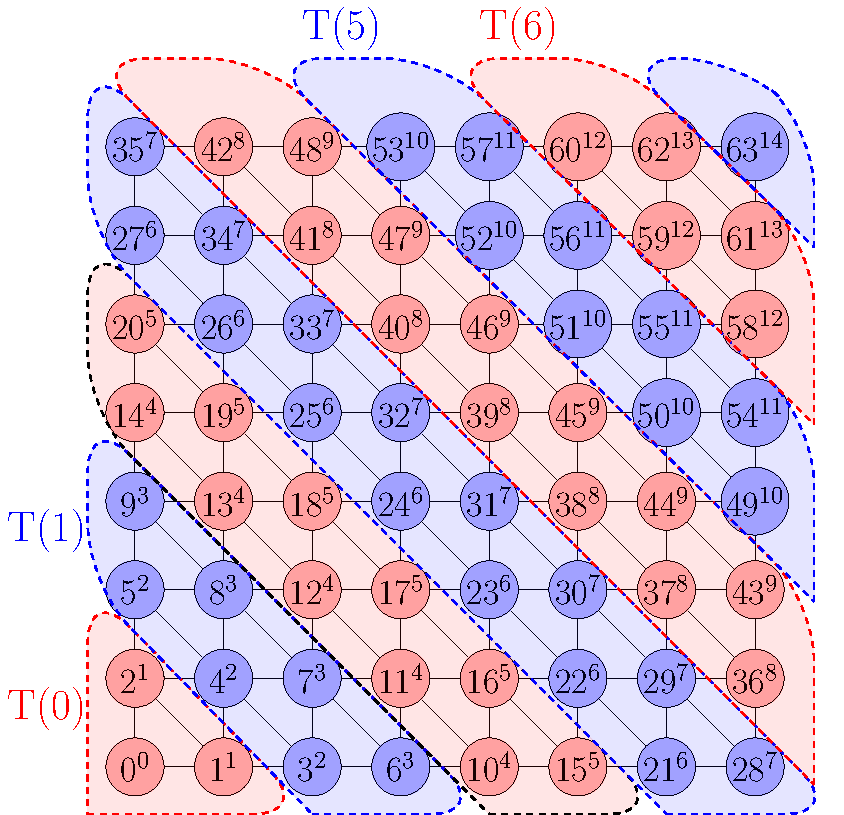
\includegraphics[scale=0.32]{pics/race_method/d2_color}}
 	\caption{\label{fig:dk_color} Example of \DONE and \DTWO coloring }
 \end{figure}
  \setlength{\belowcaptionskip}{0pt}
This criteria allows for many choices to form \DK independent levels. \Cref{fig:dk_color} shows 
one such possibility for \DONE and \DTWO coloring each. As $L(i)$ and $L(i\pm2)$ are
distance-1 independent levels, the \DONE coloring  assigns
two colors to alternating levels.  In case of \DTWO we group two adjacent levels and apply \DONE
coloring to the groups. This groups of levels are called \levelGroups
 and the $i-th$ \levelGroup is denoted as $T(i)$ (see \Cref{fig:d2_color}).
For \DONE coloring shown in \Cref{fig:d1_color} the \levels and \levelGroups
coincide ($L(i) = T(i)$).
It can be clearly seen that in both cases
 all the vertices  between \levelGroups of same color
  are \DONE/\DTWO independent  and can be executed in parallel.
   For example in case of \DTWO, \levelGroups $T(0), T(2), T(4)$
 and $T(6)$ can be executed by four threads in parallel. After synchronization the remaining 
 four blue colored \levelGroups can be executed in parallel. Note that
 within a \levelGroup/\level the vertices are computed serially without destroying
 any data locality.

However choosing same number of \levels per \levelGroup may cause severe
load imbalance depending on the matrix. For example in \Cref{fig:d2_color} 
 \levelGroups at extreme ends $T(0), T(7)$  have relatively low number of 
 vertices (proportional to computational work)  compared to the \levelGroups 
 in the middle ($T(3),T(4)$).


\subsection{Load Balancing}
\Acrshort{RACE} applies a load-balancing scheme to balance the work-load
between different threads within each color. The main idea of this step
is to incorporate hardware features like number of threads into the 
method. It does this by generating just sufficient amount of \levelGroups 
as required by the hardware and then applies a load-balancing algorithm.
The algorithm minimizes the variance between number of vertices 
within \levelGroups of the same color. \Inorder to
 accomplish this \levelGroups containing low workload (number of vertices)
 grabs adjacent \levels from neighboring \levelGroups and the overloaded
 \levelGroups shift \levels to adjacent \levelGroups. To maintain
 \DK independence between \levelGroups of same color the algorithm 
 takes care to ensure \atleast $k$ levels in a \levelGroup. The algorithm 
 does this shifting process in an iterative manner until it reaches the
 minimum possible variance or no further moves are possible due to
 \DK coloring.
 
  \setlength{\belowcaptionskip}{-10pt}
  \begin{figure}[t]
  	\begin{minipage}[c]{0.28\textwidth}
  	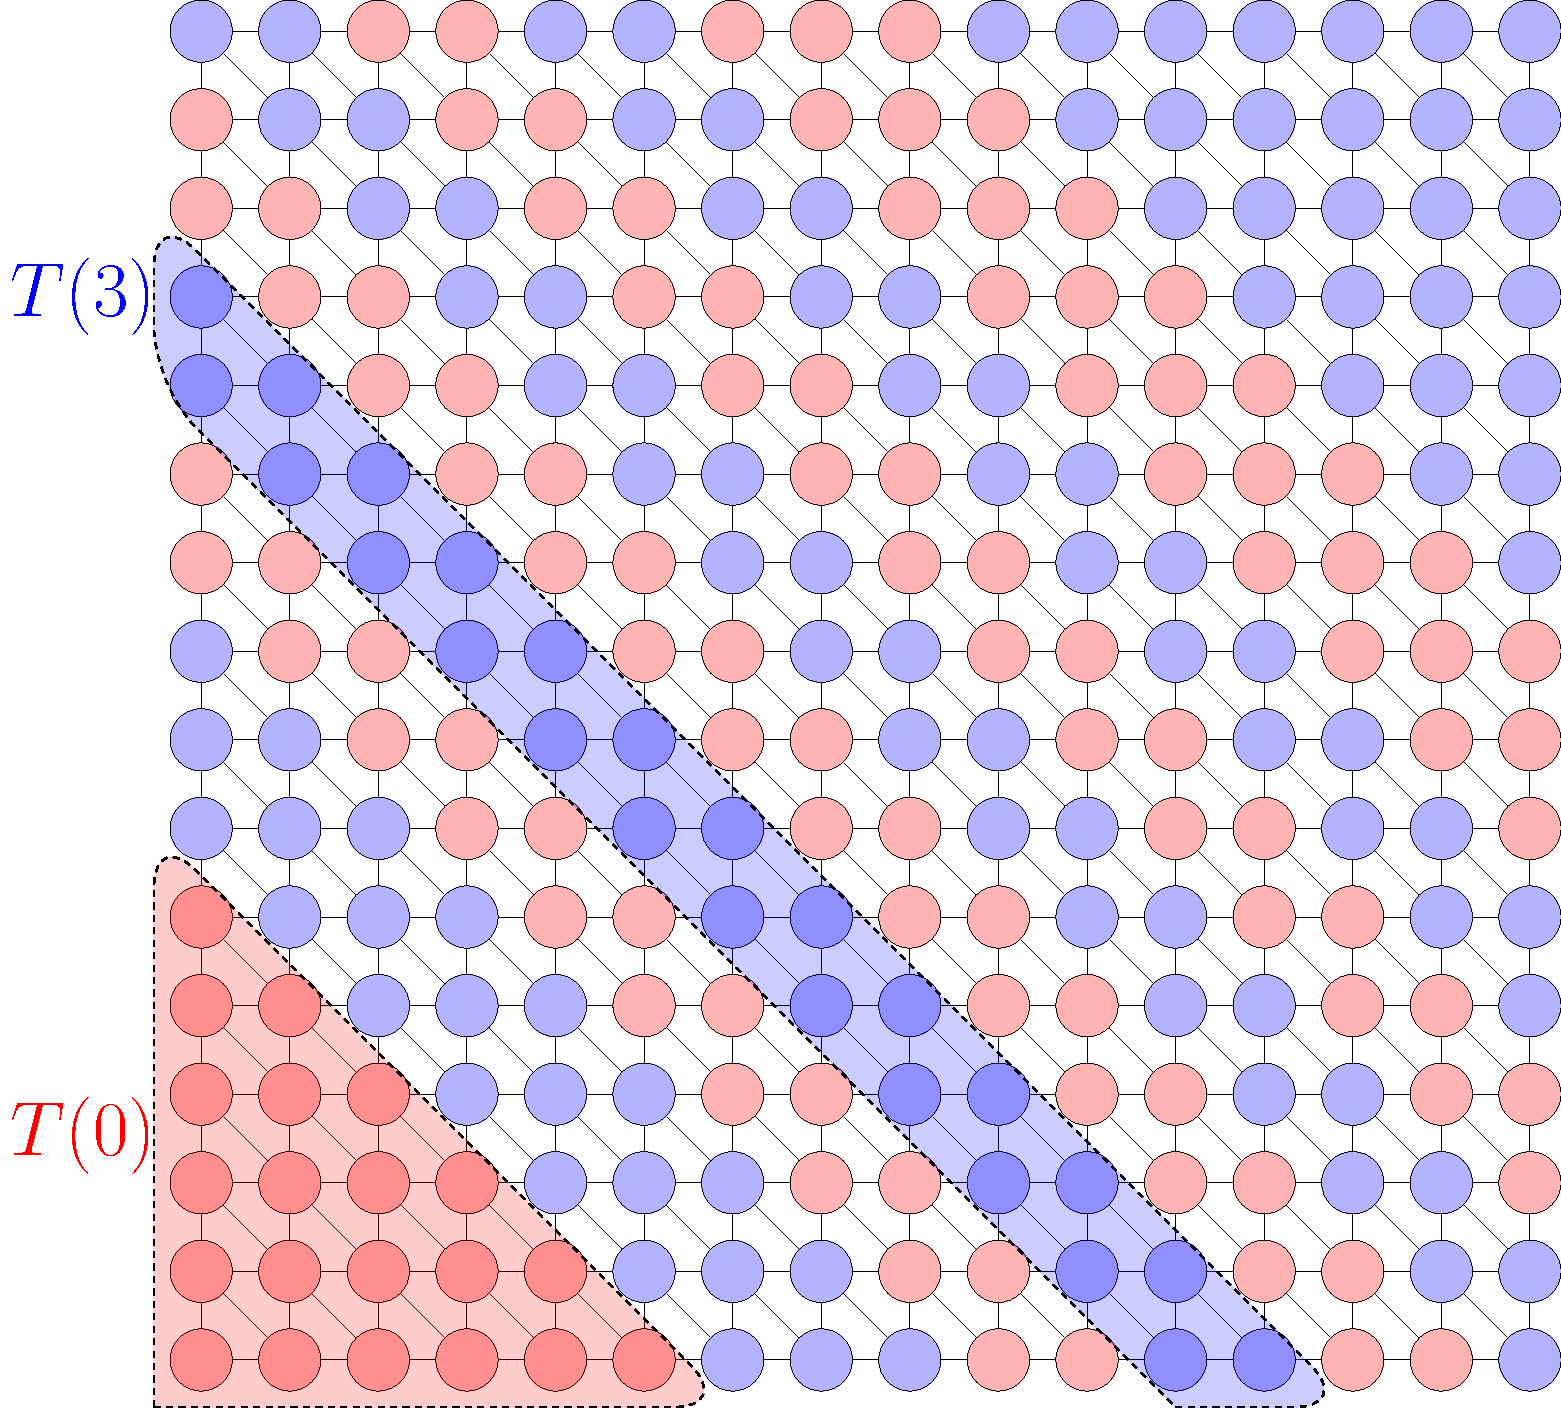
\includegraphics[height=12.4em,width=15em]{pics/race_method/load_balancing}
  	\end{minipage}\hspace{2.5em}
  	 \begin{minipage}[c]{0.14\textwidth}
  	\caption{\label{fig:lb} After load balancing for five threads and \DTWO
  		dependency on 2d-7pt example, domain size $16\times16$.  }
  	\end{minipage}
  \end{figure}
   \setlength{\belowcaptionskip}{0pt}
   
  \Cref{fig:lb} shows the graph of 2d-7pt example size $16\times16$ after
   applying the load balancing. Here \DTWO coloring and five threads
    (\ie ten \levelGroups) were the input to the load balancing algorithm.
    Note that \levelGroups at extreme ends (\eg $T(0)$) have more levels
    since here each levels have low number of vertices. While bigger \levelGroups
    (\eg $T(3)$) at middle maintain two levels to preserve \DK coloring.
    
\subsection{Recursion}

%\lipsum


\section{Results \& Contribution} \label{sec:results}
We evaluate the performance of \acrshort{RACE} by parallelizing the \acrshort{SymmSpMV}
kernel shown in \Cref{alg:symmSpMV}. This allows to get a clear picture of the
performance advantage of \acrshort{RACE} compared to other methods. Finally,
in this section we use \acrshort{RACE} to parallelize a eigenvalue solver, 
and compare it against standard approaches.

\subsection{Analysis of SymmSpMV Performance}
Matrix vector multiplication is a frequently used and time-consuming kernel in
many numerical simulations. But in most of the cases, even if the matrix is symmetric,
the full (general) matrix is used to perform these computations.
This is due to the lack of effective widely usable \acrshort{SymmSpMV} implementations available.
With the modern limited memory capacity HBM (High Bandwidth Memory) it 
is critical to use the \acrshort{SymmSpMV} kernel for achieving high performance.

Therefore in this section we carry out experiments using the \acrshort{SymmSpMV} kernel.
For this comparison we choose most of the matrices from publicly available Suite
SuiteSparse Matrix Collection \cite{UOF}, combining frequently 
used matrices in related literatures \cite{RSB,park_ls}. We also added
some matrices from quantum physics applications, which originates from 
the particular context in which \acrshort{RACE} was developed \cite{ESSEX}.
The experiments are
run on one socket of the modern \Intel \SKX (Gold 6148) architecture
clocked at 2.4 \GHZ. The reported performance is purely for the \acrshort{SymmSpMV}
computation as normally these kernels are called multiple times making other
costs (like setup time) negligible.

\begin{figure*}[tb]
	\subfloat[Performance of \acrshort{RACE} compared with MKL ]{\label{fig:race_vs_mkl}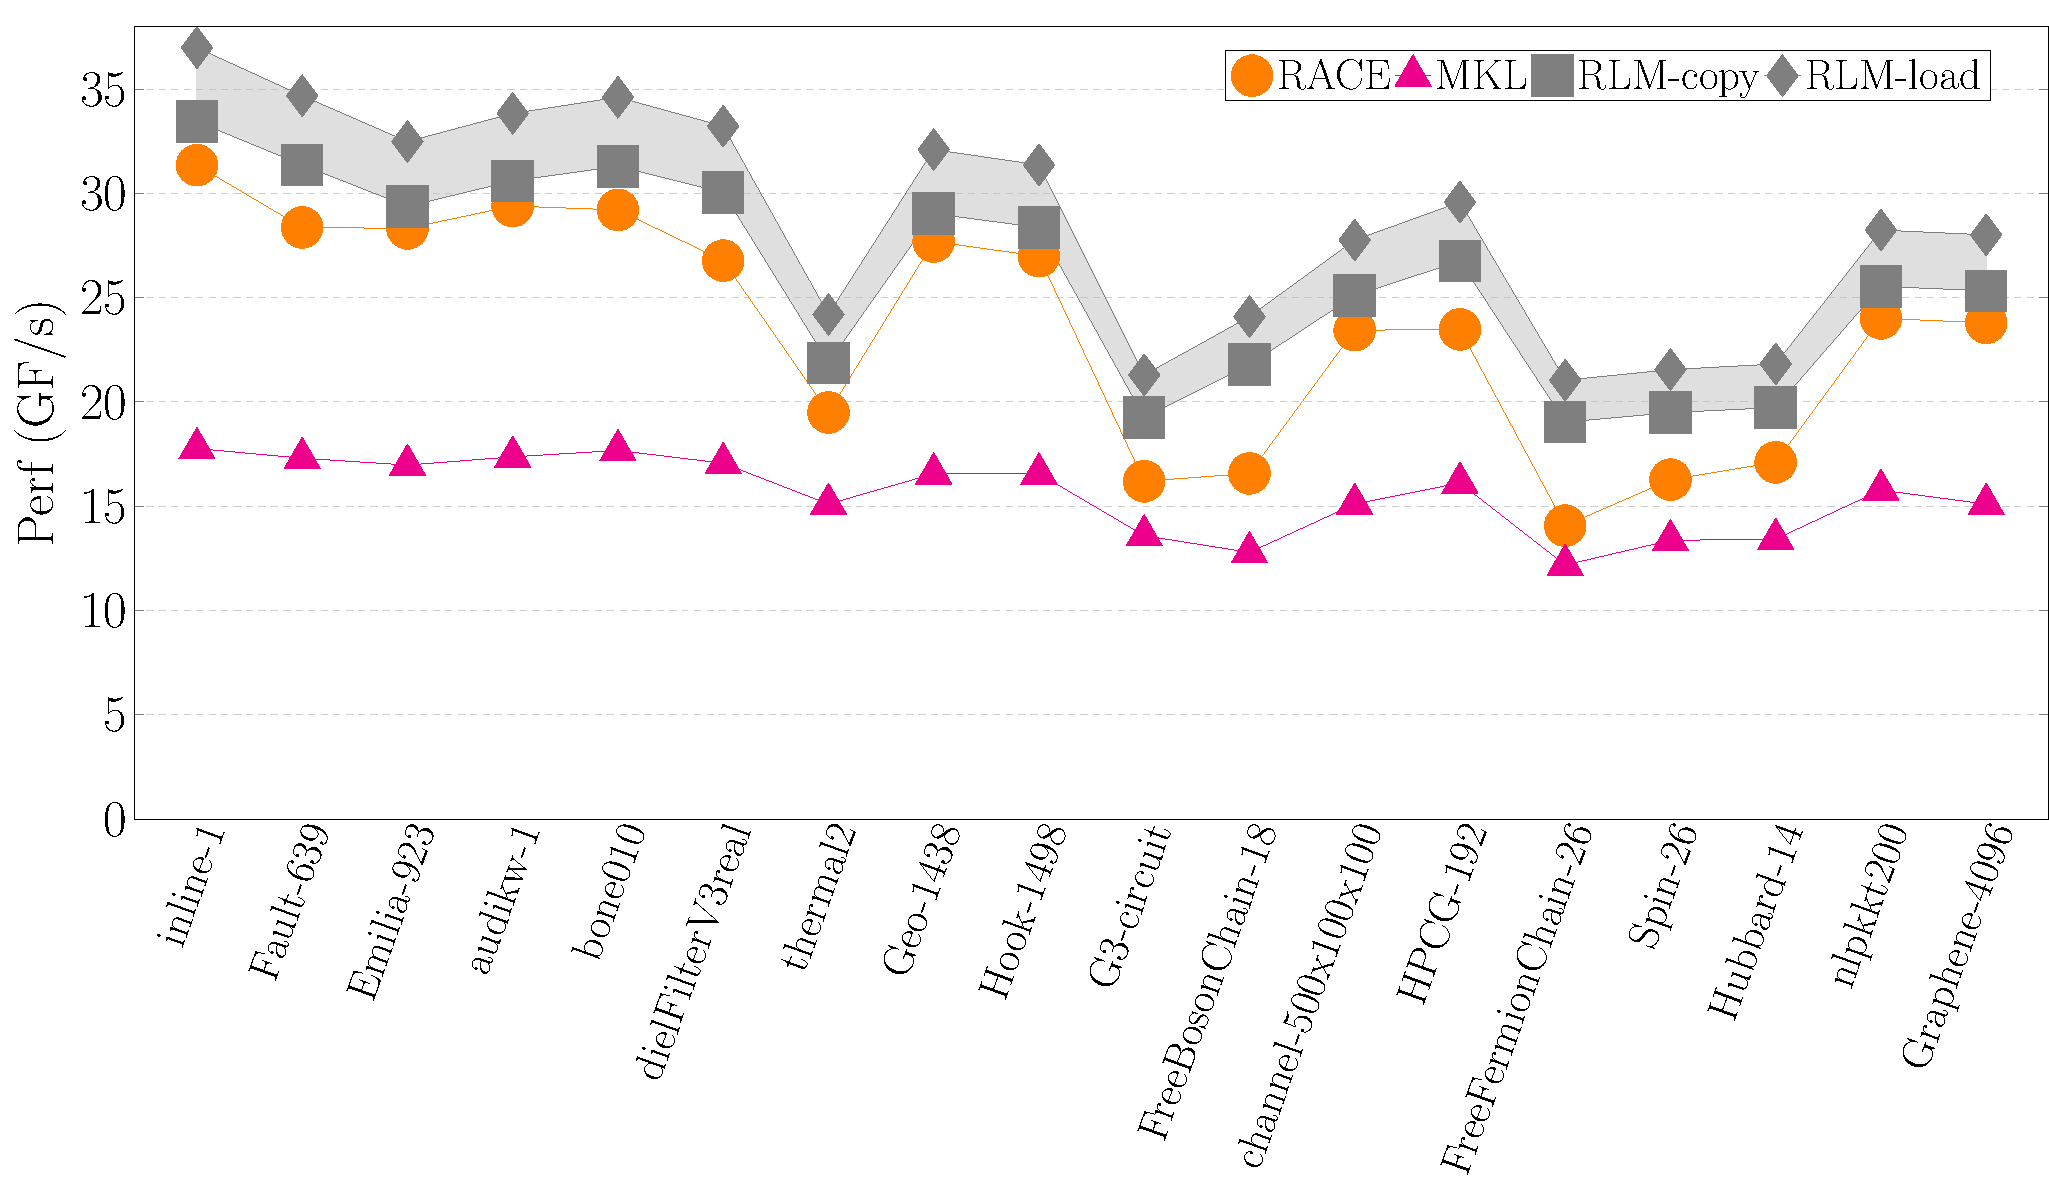
\includegraphics[scale=0.25]{pics/symm_spmv/skx/RACE_vs_MKL}}
	\subfloat[Performance of RACE compared to coloring approaches]{\label{fig:race_vs_mc}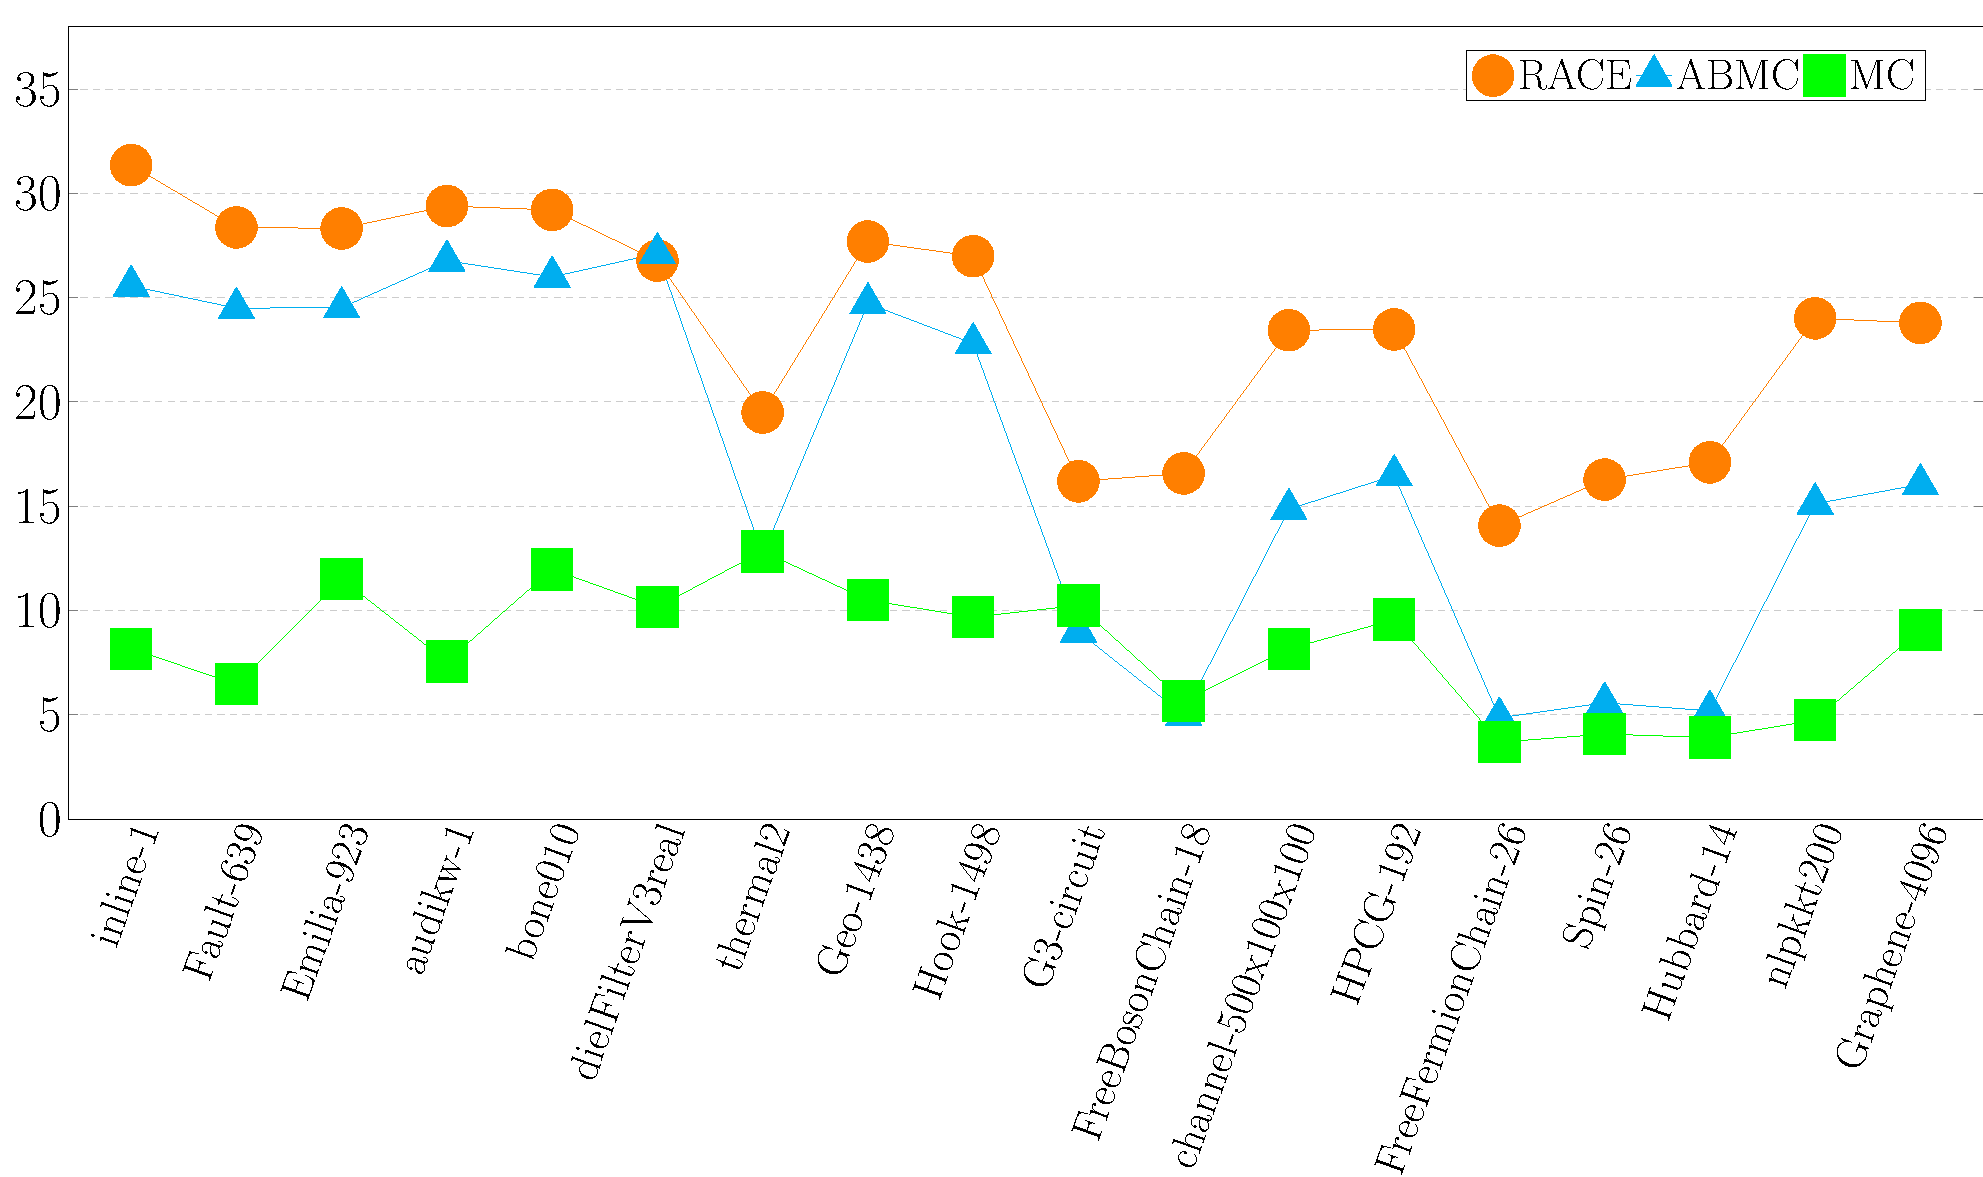
\includegraphics[scale=0.25]{pics/symm_spmv/skx/RACE_vs_MC}}
	\caption{\label{fig:symm_spmv_perf} \acrshort{SymmSpMV} performance of \acrshort{RACE} compared to 
		various methods. The performance model of \acrshort{SymmSpMV} is shown in 
		\cref{fig:race_vs_mkl} for reference. Note that the matrices are ordered according 
		to increasing number of rows.}
\end{figure*}
To establish a yardstick to compare \acrshort{RACE} performance we use 
performance modeling. The performance model is based on the Roofline  model (RLM)
 \cite{Williams_roofline}  and derived using the principles shown 
 in \cite{Moritz_sell}. The model is adjusted to suite for \acrshort{SymmSpMV}
kernel. \Cref{fig:race_vs_mkl} shows the performance of \acrshort{RACE}
on different matrices, along with the range of upper performance bounds 
(RLM-load and RLM-copy). The range corresponds to models derived using two
extreme cases of memory bandwidths observed on this processor. \CAcomm{Is it better to show only copy?}
We see that in almost all the cases the \acrshort{SymmSpMV} implementation
using \acrshort{RACE} attains higher than $85\%$ of the maximum achievable performance.
This is made possible since \acrshort{RACE} is able to preserve good data
locality and have minimal data traffic, which we have already seen in
 \Cref{fig:motivation_data} for the \texttt{Spin-26} matrix. 
 
%Next we compare the \acrshort{RACE} method with other approaches. 
In \Cref{fig:race_vs_mkl} we compare it against the \acrshort{SymmSpMV} 
implementation of a widely used numerical library, the \acrshort{MKL}. 
We use the latest implementation of MKL, which uses the Inspector-Executor routines.
The comparisons show that \acrshort{RACE} outperforms MKL
versions by a factor of $1.5\times$ in average. A simple analysis
shows that the performance of the \acrshort{MKL} \acrshort{SymmSpMV} 
kernel coincides with the matrix vector multiplication using the full
matrix (\acrshort{SpMV}), which indicates that MKL might be converting
the symmetric matrix to a full matrix internally and doing a general \acrshort{SpMV}
operation. However as MKL being closed source  the algorithm 
used to parallelize the code is unknown.

Further we compare the \acrshort{RACE} method with the two widely used
coloring methods. For \acrshort{MC} method we apply \acrlong{MC} scheme
generated by the COLPACK \cite{COLPACK} library to parallelize the \acrshort{SymmSpMV}
kernel. In the \acrshort{ABMC} method we first partition the matrix into blocks
using METIS \cite{METIS} and apply coloring using the \COLPACK library. The
size of blocks was determined by a parameter scan (range 4 \ldots 128, see \cite{ABMC}).
\Cref{fig:race_vs_mc} compares the performance of \acrshort{RACE} with the other 
two coloring approaches.
Overall \acrshort{MC} method is not competitive, while \acrshort{ABMC} delivers
modest performance ($80 \%$ of \acrshort{RACE}) for small matrices. But for large
matrices,  where data locality plays a vital role \acrshort{ABMC} 
falls substantially behind \acrshort{RACE} as the indirectly
accessed vectors no more fit in cache. To make this comparison easier
the matrices are arranged according to increasing number of rows.
Overall \acrshort{RACE} has an average speedup of $1.6\times$ compared to 
\acrshort{ABMC} method, while in some cases speedup can be as high as $3\times$.


%First we establish performance model for 
%\acrshort{SymmSpMV} and compare it to \acrshort{RACE} performance to estimate
%the quality of our method. Then we compare \acrshort{RACE} with the
%two coloring approaches introduced before and the 

\begin{itemize}
	\item Test setup, brief is sufficient
	\item Start with Spin matrix, and little RLM
	\item SymmSpMV performance
\end{itemize}


\subsection{FEAST with RACE}
\lipsum
\begin{figure}[tb]
	\centering
	\scalebox{0.56}{%\documentclass{standalone}
%\usepackage{tikz}
%\usepackage{pgfplots}

%\usepackage{comment}
%\usepackage{filecontents}

\pgfplotsset{width=7.5cm,height=8.75cm,compat=1.3}
%\begin{filecontents}{data_mkl.dat}
%size, nrows,   Time,		Mem		
%40,		64000,	9.92,		968724
%60,		216000,	76.31,	2739456
%70,		343000,	 230.26,	5066384 
%80,		512000, 452.685, 7670076
%120,	1728000, 6600.29, 36152256
%140, 	2744000, 16473.6, 65311968
%\end{filecontents}

%\begin{filecontents}{data_cgmn.dat}
%size, nrows,   Time,		Mem		
%40,		64000,	78.99,	332364
%60,		216000,	1007,  661684
%70,		343000,	 2277.09,  959544
%80,		512000, 4302.18, 1440628
%120,	1728000, 29777.8, 4106652
%140, 	2744000, 57916.9, 6316176
%160,	4096000, 118008, 9379604
%220,	10648000, 527629.5, 23632788
%\end{filecontents}


%\begin{document}

\begin{tikzpicture}


  \def\xmin{0}
  \def\xmax{10}
  \def\ymin{0}
  \def\ymax{30}

  \begin{axis}[ xlabel={Size (n)}, ylabel={Time(s)}, ymode=linear,
  xtick={ 64000, 125000, 216000, 512000,   1728000, 5832000, 15625000 },
  xticklabels={$40^3$
    , $50^3$, $60^3$,  $80^3$,   $120^3$, $180^3$, $250^3$ },
  ytick={ 100, 1000, 10000, 100000,   1000000},
  yticklabels={$10^2$
  	, $10^3$, $10^4$,  $10^5$,   $10^6$ },
  scaled ticks=false,
  xmode=log,
  ymode=log,
  ymax=100000000,
 % xmin=27000,xmax = 15625000,
  %ymin=0, ymax=14,
  legend style={legend pos=north west}]

   \addplot+[mark=square*, mark size=2pt, mark options={magenta}, draw=magenta, line width=1.5] table[x expr=\thisrow{size}*\thisrow{size}*\thisrow{size},y expr=\thisrow{Time},col sep=comma] {pics/feast/skx/data_mkl.dat}; \label{plot_one}
   \addlegendentry{Intel MKL(Pardiso)}

   \addplot+[mark=*, mark size=2pt, mark options={orange}, draw=orange, line width=1.5] table[x expr=\thisrow{size}*\thisrow{size}*\thisrow{size},y expr=\thisrow{Time},col sep=comma] {pics/feast/skx/data_cgmn.dat}; \label{plot_two}
   \addlegendentry{RACE-CGMN}

	\addplot+[mark=triangle*, mark size=2pt, mark options={cyan}, draw=cyan, line width=1.5 ] table[x expr=\thisrow{size}*\thisrow{size}*\thisrow{size},y expr=\thisrow{Time},col sep=comma] {pics/feast/skx/data_cgmn_abmc.dat}; \label{plot_three}
	\addlegendentry{ABMC-CGMN}

   \addplot+[mark=none, mark options={magenta}, draw=magenta, line width=1, dashed] table[x = nrows,y expr=76.3
   *(\thisrow{nrows}/60^3)^2.12,col sep=comma] {pics/feast/skx/data_proj.dat}; \label{plot_three}
   \addlegendentry{$\mathcal{O}(n^{2})$}
   
   \addplot+[mark=none,  mark options={orange}, draw=orange, line width=1, dashed] table[x = nrows,y expr=1050*(\thisrow{nrows}/60^3)^1.57,col sep=comma] {pics/feast/skx/data_proj.dat}; \label{plot_four}
   \addlegendentry{$\mathcal{O}(n^{1.56})$}
   
   %\addplot table[x index=1,y index=4,col sep=comma] {data_mkl.dat}; \label{plot_three}
   %\addlegendentry{Flops DP}

 \end{axis}

\end{tikzpicture}

%\end{document}}
	%	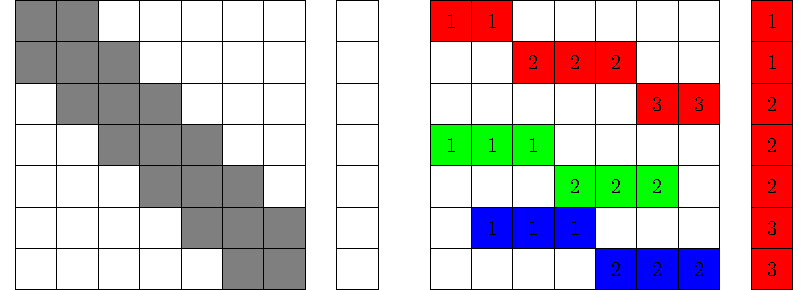
\includegraphics[scale=0.6]{pics/alpha_problem/mc_alpha_unsymm_only_red.tex}
	\caption{Comparison of FEAST with default \acrshort{MKL} direct solver and 
		iterative solver CGMN parallelized using \acrshort{RACE}. The experiment is
		run on one socket of \SKX (Platinum 8160) chip. Please note both x and y axes
		are in log scale.}
\end{figure}

\begin{itemize}
	\item Briefly describe FEAST
	\item Tell its implemented in MKL, we use Reverse Communication Interface (RCI) of
		\acrshort{MKL} to implement inner linear solver
	\item Tell why we need KACZ -> ill-conditioned linear system, robustness of KACZ -> only potential iterative solver. Tell 99\% of time it uses in this CGMN solver
	\item To our knowledge first implementation that uses iterative inner linear system, which is really inevitable to scale and for large size problems
	\item  Test setup, discrete laplacian, 10 inner eigenvalues, complex numbers 
	\item Comparison with default Pardiso
	\item Discuss on Big O ....
\end{itemize}


\section{Future Work}

\begin{acks}
\begin{itemize}
	\item Georg, Olaf, Jonas, Thomas Gruber
	\item RRZE and RWTH for providing computations time.
\end{itemize}
\end{acks}


